\documentclass[11pt,oneside]{article}
\usepackage[T1]{fontenc}
\usepackage[utf8]{inputenc}
% \usepackage{lmodern}
%\usepackage[adobe-utopia,uppercase=upright,greeklowercase=upright]{mathdesign}
\usepackage[adobe-utopia]{mathdesign}
%\usepackage{minionpro}
% \usepackage{pifont}
% \usepackage{amssymb}
\usepackage{amsmath}
\usepackage[francais]{babel}
% \usepackage[francais]{varioref}
\usepackage[dvips]{graphicx}

\usepackage{framed}
\usepackage[normalem]{ulem}
\usepackage{fancyhdr}
\usepackage{titlesec}
\usepackage{vmargin}
\usepackage{longtable}

\usepackage{ifthen}


%\usepackage{epsfig}
\usepackage{subfig}

\usepackage{multirow}
\usepackage{multicol} % Portions de texte en colonnes
\usepackage{flafter}%floatants après la référence



\usepackage{color}
\usepackage{colortbl}


\definecolor{gris25}{gray}{0.75}
\definecolor{bleu}{RGB}{18,33,98}
\definecolor{bleuf}{RGB}{42,94,171}
\definecolor{bleuc}{RGB}{231,239,247}
\definecolor{rougef}{RGB}{185,18,27}
\definecolor{rougec}{RGB}{255,230,231}
\definecolor{vertf}{RGB}{103,126,82}
\definecolor{vertc}{RGB}{220,255,191}
\definecolor{violetf}{RGB}{112,48,160}
\definecolor{violetc}{RGB}{230,224,236}

\newenvironment{sci}[1][\hsize]%
{%
    \def\FrameCommand%
    {%
%\rotatebox{90}{\textit{\textsf{Scilab}}
\includegraphics[height=.8cm]{png/logo_scilab}} 
\rotatebox{90}{
\includegraphics[height=.6cm]{png/logo_scilab}} 
        {\color{violetf}\vrule width 3pt}%
        \hspace{0pt}%must no space.
        \fboxsep=\FrameSep\colorbox{violetc}%
    }%
    \MakeFramed{\hsize #1 \advance\hsize-\width\FrameRestore}%
}%
{\endMakeFramed}%

\newenvironment{pseudo}[1][\hsize]%
{%
    \def\FrameCommand%
    {%
\rotatebox{90}{\textit{\textsf{Pseudo Code}}} 
        {\color{violetf}\vrule width 3pt}%
        \hspace{0pt}%must no space.
        \fboxsep=\FrameSep\colorbox{violetc}%
    }%
    \MakeFramed{\hsize #1 \advance\hsize-\width\FrameRestore}%
}%
{\endMakeFramed}%

\newenvironment{py}[1][\hsize]%
{%
    \def\FrameCommand%
    {%
%\rotatebox{90}{\textit{\textsf{Python}}} 
\rotatebox{90}{
\includegraphics[height=.6cm]{png/logo_python}} 
        {\color{violetf}\vrule width 3pt}%
        \hspace{0pt}%must no space.
        \fboxsep=\FrameSep\colorbox{violetc}%
    }%
    \MakeFramed{\hsize #1 \advance\hsize-\width\FrameRestore}%
}%
{\endMakeFramed}%


\newenvironment{corrige}[1][\hsize]%
{%
    \def\FrameCommand
    {%
\rotatebox{90}{\textit{\textsf{Correction}}} 
        {\color{violetf}\vrule width 3pt}%
        \hspace{0pt}%must no space.
        \fboxsep=\FrameSep\colorbox{violetc}%
    }%
    \MakeFramed{\hsize#1\advance\hsize-\width\FrameRestore}%
}%
{\endMakeFramed}%



\newenvironment{rem}[1][\hsize]%
{%
    \def\FrameCommand
    {%
\rotatebox{90}{\textit{\textsf{Remarque}}} 
        {\color{bleuf}\vrule width 3pt}%
        \hspace{0pt}%must no space.
        \fboxsep=\FrameSep\colorbox{bleuc}%
    }%
    \MakeFramed{\hsize#1\advance\hsize-\width\FrameRestore}%
}%
{\endMakeFramed}%


\newenvironment{savoir}[1][\hsize]%
{%
    \def\FrameCommand
    {%
\rotatebox{90}{\textit{\textsf{Savoir}}} 
        {\color{bleuf}\vrule width 3pt}%
        \hspace{0pt}%must no space.
        \fboxsep=\FrameSep\colorbox{bleuc}%
    }%
    \MakeFramed{\hsize#1\advance\hsize-\width\FrameRestore}%
}%
{\endMakeFramed}%

\newenvironment{prob}[1][\hsize]%
{%
    \def\FrameCommand%
    {%
\rotatebox{90}{\textit{\textsf{ Problématique}}} 
        {\color{rougef}\vrule width 3pt}%
        \hspace{0pt}%must no space.
        \fboxsep=\FrameSep\colorbox{rougec}%
    }%
    \MakeFramed{\hsize#1\advance\hsize-\width\FrameRestore}%
}%
{\endMakeFramed}%

\newenvironment{obj}[1][\hsize]%
{%
    \def\FrameCommand%
    {%
\rotatebox{90}{\textit{\textsf{Objectifs}}} 
        {\color{rougef}\vrule width 3pt}%
        \hspace{0pt}%must no space.
        \fboxsep=\FrameSep\colorbox{rougec}%
    }%
    \MakeFramed{\hsize#1\advance\hsize-\width\FrameRestore}%
}%
{\endMakeFramed}%

\newenvironment{defi}[1][\hsize]%
{%
    \def\FrameCommand%
    {%
\rotatebox{90}{\textit{\textsf{Définition\\}}} 
        {\color{bleuf}\vrule width 3pt}%
        \hspace{0pt}%must no space.
        \fboxsep=\FrameSep\colorbox{bleuc}%
    }%
    \MakeFramed{\hsize#1\advance\hsize-\width\FrameRestore}%
}%
{\endMakeFramed}%


\newenvironment{demo}[1][\hsize]%
{%
    \def\FrameCommand%
    {%
\rotatebox{90}{\textit{\textsf{Démonstration\\}}} 
        {\color{bleuf}\vrule width 3pt}%
        \hspace{0pt}%must no space.
        \fboxsep=\FrameSep\colorbox{bleuc}%
    }%
    \MakeFramed{\hsize#1\advance\hsize-\width\FrameRestore}%
}%
{\endMakeFramed}%


\newenvironment{hypo}[1][\hsize]%
{%
    \def\FrameCommand%
    {%
\rotatebox{90}{\textit{\textsf{Hypothèse\\}}} 
        {\color{bleuf}\vrule width 3pt}%
        \hspace{0pt}%must no space.
        \fboxsep=\FrameSep\colorbox{bleuc}%
    }%
    \MakeFramed{\hsize#1\advance\hsize-\width\FrameRestore}%
}%
{\endMakeFramed}%


\newenvironment{prop}[1][\hsize]%
{%
    \def\FrameCommand%
    {%
\rotatebox{90}{\textit{\textsf{Propriété\\}}} 
        {\color{bleuf}\vrule width 3pt}%
        \hspace{0pt}%must no space.
        \fboxsep=\FrameSep\colorbox{bleuc}%
    }%
    \MakeFramed{\hsize#1\advance\hsize-\width\FrameRestore}%
}%
{\endMakeFramed}%

\newenvironment{props}[1][\hsize]%
{%
    \def\FrameCommand%
    {%
\rotatebox{90}{\textit{\textsf{Propriétés\\}}} 
        {\color{bleuf}\vrule width 3pt}%
        \hspace{0pt}%must no space.
        \fboxsep=\FrameSep\colorbox{bleuc}%
    }%
    \MakeFramed{\hsize#1\advance\hsize-\width\FrameRestore}%
}%
{\endMakeFramed}%

\newenvironment{exemple}[1][\hsize]%
{%
    \def\FrameCommand%
    {%
\rotatebox{90}{\textit{\textsf{Exemple\\}}} 
        {\color{vertf}\vrule width 3pt}%
        \hspace{0pt}%must no space.
        \fboxsep=\FrameSep\colorbox{vertc}%
    }%
    \MakeFramed{\hsize#1\advance\hsize-\width\FrameRestore}%
}%
{\endMakeFramed}%

\newenvironment{resultat}[1][\hsize]%
{%
    \def\FrameCommand%
    {%
\rotatebox{90}{\textit{\textsf{Résultat\\}}} 
        {\color{rougef}\vrule width 3pt}%
        \hspace{0pt}%must no space.
        \fboxsep=\FrameSep\colorbox{rougec}%
    }%
    \MakeFramed{\hsize#1\advance\hsize-\width\FrameRestore}%
}%
{\endMakeFramed}%

\newenvironment{methode}[1][\hsize]%
{%
    \def\FrameCommand%
    {%
\rotatebox{90}{\textit{\textsf{Méthode\\}}} 
        {\color{rougef}\vrule width 3pt}%
        \hspace{0pt}%must no space.
        \fboxsep=\FrameSep\colorbox{rougec}%
    }%
    \MakeFramed{\hsize#1\advance\hsize-\width\FrameRestore}%
}%
{\endMakeFramed}%

\newenvironment{theo}[1][\hsize]%
{%
    \def\FrameCommand%
    {%
\rotatebox{90}{\textit{\textsf{Théorème\\}}} 
        {\color{rougef}\vrule width 3pt}%
        \hspace{0pt}%must no space.
        \fboxsep=\FrameSep\colorbox{rougec}%
    }%
    \MakeFramed{\hsize#1\advance\hsize-\width\FrameRestore}%
}%
{\endMakeFramed}%

\newenvironment{warn}[1][\hsize]%
{%
    \def\FrameCommand%
    {%
\rotatebox{90}{\textit{\textsf{Attention\\}}} 
        {\color{rougef}\vrule width 3pt}%
        \hspace{0pt}%must no space.
        \fboxsep=\FrameSep\colorbox{rougec}%
    }%
    \MakeFramed{\hsize#1\advance\hsize-\width\FrameRestore}%
}%
{\endMakeFramed}%

% \usepackage{pstricks}
%\usepackage{minitoc}
% \setcounter{minitocdepth}{4}

\setcounter{tocdepth}{2}

% \mtcselectlanguage{french} 

%\usepackage{draftcopy}% "Brouillon"
% \usepackage{floatflt}
\usepackage{psfrag}
%\usepackage{listings} % Permet d'insérer du code de programmation
\renewcommand{\baselinestretch}{1.2}

% Changer la numérotation des figures :
% ------------------------------------
% \makeatletter
% \renewcommand{\thefigure}{\ifnum \c@section>\z@ \thesection.\fi
%  \@arabic\c@figure}
% \@addtoreset{figure}{section}
% \makeatother
 


%%%%%%%%%%%%
% Définition des vecteurs %
%%%%%%%%%%%%
 \newcommand{\vect}[1]{\overrightarrow{#1}}

%%%%%%%%%%%%
% Définition des torseusr %
%%%%%%%%%%%%

 \newcommand{\torseur}[1]{%
\left\{{#1}\right\}
}

\newcommand{\torseurcin}[3]{%
\left\{\mathcal{#1} \left(#2/#3 \right) \right\}
}

\newcommand{\torseurstat}[3]{%
\left\{\mathcal{#1} \left(#2\rightarrow #3 \right) \right\}
}

 \newcommand{\torseurc}[8]{%
%\left\{#1 \right\}=
\left\{
{#1}
\right\}
 = 
\left\{%
\begin{array}{cc}%
{#2} & {#5}\\%
{#3} & {#6}\\%
{#4} & {#7}\\%
\end{array}%
\right\}_{#8}%
}

 \newcommand{\torseurcol}[7]{
\left\{%
\begin{array}{cc}%
{#1} & {#4}\\%
{#2} & {#5}\\%
{#3} & {#6}\\%
\end{array}%
\right\}_{#7}%
}

 \newcommand{\torseurl}[3]{%
%\left\{\mathcal{#1}\right\}_{#2}=%
\left\{%
\begin{array}{l}%
{#1} \\%
{#2} %
\end{array}%
\right\}_{#3}%
}

 \newcommand{\vectv}[3]{%
\vect{V\left( {#1} \in {#2}/{#3}\right)}
}


\newcommand{\vectf}[2]{%
\vect{R\left( {#1} \rightarrow {#2}\right)}
}

\newcommand{\vectm}[3]{%
\vect{\mathcal{M}\left( {#1}, {#2} \rightarrow {#3}\right)}
}


 \newcommand{\vectg}[3]{%
\vect{\Gamma \left( {#1} \in {#2}/{#3}\right)}
}

 \newcommand{\vecto}[2]{%
\vect{\Omega\left( {#1}/{#2}\right)}
}
% }$$\left\{\mathcal{#1} \right\}_{#2} =%
% \left\{%
% \begin{array}{c}%
%  #3 \\%
%  #4 %
% \end{array}%
% \right\}_{#5}}

%  ------------------------------------------
% | Modification du formatage des sections : | 
%  ------------------------------------------

% Grands titres :
% ---------------

\newcommand{\titre}[1]{%
\begin{center}
      \bigskip
      \rule{\textwidth}{1pt}
      \par\vspace{0.1cm}
      
      \textbf{\large #1}
      \par\rule{\textwidth}{1pt}
    \end{center}
    \bigskip
  }

% Supprime le numéro du chapitre dans la numérotation des sections:
% -----------------------------------------------------------------
\makeatletter
\renewcommand{\thesection}{\@arabic\c@section}
\makeatother


% \titleformat{\chapter}[display]
% {\normalfont\Large\filcenter}
% {}
% {1pc}
% {\titlerule[1pt]
%   \vspace{1pc}%
%   \Huge}[\vspace{1ex}%
% \titlerule]


%%%% Chapitres Comme PY Pechard %%%%%%%%%
% numéro du chapitre
\DeclareFixedFont{\chapnumfont}{OT1}{phv}{b}{n}{80pt}
% pour le mot « Chapitre »
\DeclareFixedFont{\chapchapfont}{OT1}{phv}{m}{it}{40pt}
% pour le titre
\DeclareFixedFont{\chaptitfont}{T1}{phv}{b}{n}{25pt}

\definecolor{gris}{gray}{0.75}
\titleformat{\chapter}[display]%
	{\sffamily}%
	{\filleft\chapchapfont\color{gris}\chaptertitlename\
	\\
	\vspace{12pt}
	\chapnumfont\thechapter}%
	{16pt}%
	{\filleft\chaptitfont}%
	[\vspace{6pt}\titlerule\titlerule\titlerule]

%%%%  Fin Chapitres Comme PY Pechard %%%%%%%%%


% Section, subsection, subsubsection sans serifs :
% % ----------------------------------------------

% \makeatletter
% \renewcommand{\section}{\@startsection{section}{0}{0mm}%
% {\baselineskip}{.3\baselineskip}%
% {\normalfont\sffamily\Large\textbf}}%
% \makeatother

\makeatletter
\renewcommand{\@seccntformat}[1]{{\textcolor{bleu}{\csname
the#1\endcsname}\hspace{0.5em}}}
\makeatother

\makeatletter
\renewcommand{\section}{\@startsection{section}{1}{\z@}%
                       {-4ex \@plus -1ex \@minus -.4ex}%
                       {1ex \@plus.2ex }%
                       {\normalfont\Large\sffamily\bfseries}}%
\makeatother
 
\makeatletter
\renewcommand{\subsection}{\@startsection {subsection}{2}{\z@}
                          {-3ex \@plus -0.1ex \@minus -.4ex}%
                          {0.5ex \@plus.2ex }%
                          {\normalfont\large\sffamily\bfseries}}
\makeatother
 
\makeatletter
\renewcommand{\subsubsection}{\@startsection {subsubsection}{3}{\z@}
                          {-2ex \@plus -0.1ex \@minus -.2ex}%
                          {0.2ex \@plus.2ex }%
                          {\normalfont\large\sffamily\bfseries}}
\makeatother
 
\makeatletter             
\renewcommand{\paragraph}{\@startsection{paragraph}{4}{\z@}%
                                    {-2ex \@plus-.2ex \@minus .2ex}%
                                    {0.1ex}%               
{\normalfont\sffamily\bfseries}}
\makeatother
 

\makeatletter             
\renewcommand{\subparagraph}{\@startsection{subparagraph}{5}{\z@}%
                                    {-2ex \@plus-.2ex \@minus .2ex}%
                                    {0.1ex}%               
{\normalfont\bfseries Question }}
\makeatother

\renewcommand{\thesubparagraph}{\arabic{subparagraph}} 
\makeatletter

\setcounter{secnumdepth}{5}
%\renewcommand{\subparagraph}{\@startsection{subparagraph}{5}{\z@}%
%                                       {-2ex \@plus-.1ex \@minus .2ex}%
%                                       {0.1ex}%
%				    {\normalfont\normalsize\sffamily\bfseries}}
%\makeatletter
% \makeatletter
% \renewcommand{\subsection}{\@startsection{subsection}{1}{2mm}%
% {\baselineskip}{.3\baselineskip}%
% {\normalfont\sffamily\large\textbf}}%
% \makeatother
% 
% \makeatletter
% \renewcommand{\subsubsection}{\@startsection{subsubsection}{2}{4mm}%
% {\baselineskip}{.15\baselineskip}%
% {\normalfont\sffamily\large\textbf}}%
% \makeatother
% 
% \makeatletter
% \renewcommand{\paragraph}{\@startsection{paragraph}{3}{6mm}%
% {\baselineskip}{.15\baselineskip}%
% {\normalfont\sffamily\large\textbf}}%
% \makeatother
 



%  --------
% | Marges |
%  --------


% \setmarginsrb{2.5cm}{1.5cm}{2.5cm}{2cm}{1cm}{1cm}{1cm}{1cm}
\setmarginsrb{1.5cm}{1cm}{1cm}{1.5cm}{1cm}{1cm}{1cm}{1cm}

% Changer les marges localement :
% -----------------------------
\newenvironment{changemargin}[2]{\begin{list}{}{%
\setlength{\topsep}{0pt}%
\setlength{\leftmargin}{0pt}%
\setlength{\rightmargin}{0pt}%
\setlength{\listparindent}{\parindent}%
\setlength{\itemindent}{\parindent}%
\setlength{\parsep}{0pt plus 1pt}%
\addtolength{\leftmargin}{#1}%
\addtolength{\rightmargin}{#2}%
}\item }{\end{list}}



\usepackage{pst-solides3d}
\usepackage{titletoc}
\titlecontents{chapter}[+3pc]
  {\addvspace{10pt}\sffamily\bfseries}
{\contentslabel[{\pscirclebox[fillstyle=solid,fillcolor=gray!25,
linecolor=gray!25,framesep=4pt]{\textcolor{white}{\thecontentslabel}}}]{2.5pc}}
  {}
  {\dotfill \normalfont\thecontentspage\ }

\titlecontents{section}[3pc]
  {\addvspace{2pt}\sffamily}
  {\contentslabel[\thecontentslabel]{1.8pc}}
  {}
  {\dotfill \normalfont\thecontentspage\ }

\titlecontents{subsection}[5pc]
  {\addvspace{2pt}\sffamily}
  {\contentslabel[\thecontentslabel]{1.8pc}}
  {}
  {\dotfill \normalfont\thecontentspage\ }

\titlecontents{subsubsection}[8pc]
  {\addvspace{2pt}\sffamily}
  {\contentslabel[\thecontentslabel]{3pc}}
  {}
  {\dotfill \normalfont\thecontentspage\ }
%{\;\titlerule\;\normalfont\thecontentspage\ }

\titlecontents{paragraph}[9pc]
  {\addvspace{2pt}\sffamily}
  {\contentslabel[\thecontentslabel]{3.5pc}}
  {}
  {\dotfill \normalfont\thecontentspage\ }




%Si le boolen xp est vrai : compilation pour xabi
%Sinon compilation Damien
\newboolean{xp}
\setboolean{xp}{true}

\newboolean{prof}
\setboolean{prof}{false}

\def\xxtitre{\ifthenelse{\boolean{xp}}{
CI 3 -- CIN : Étude du comportement cinématique des systèmes}{
}}

\def\xxsoustitre{\ifthenelse{\boolean{xp}}{
Devoir Surveillé 7}{
}}


\def\xxauteur{\ifthenelse{\boolean{xp}}{
\noindent 2013 -- 2014 \\
Xavier \textsc{Pessoles}}{
}}


\def\xxpied{\ifthenelse{\boolean{xp}}{
Cinématique \& SLCI \\
DS 7 : \ifthenelse{\boolean{prof}}{Corrigé}{Sujet}%
}{
}}

\usepackage[%
    pdftitle={Cinématique - DS},
    pdfauthor={Xavier Pessoles},
    colorlinks=true,
    linkcolor=blue,
    citecolor=magenta]{hyperref}



\usepackage{pifont}
\sloppy
\hyphenpenalty 10000


\begin{document}






% \makeatletter \let\ps@plain\ps@empty \makeatother
%% DEBUT DU DOCUMENT
%% =================




%------------- En tetes et Pieds de Pages ------------


\pagestyle{fancy}
\ifthenelse{\boolean{xp}}{%
\renewcommand{\headrulewidth}{0pt}}{%
\renewcommand{\headrulewidth}{0.2pt}} %pour mettre le trait en haut
%\renewcommand{\headrulewidth}{0.2pt}

\fancyhead{}
\fancyhead[L]{%
\ifthenelse{\boolean{xp}}{%
\noindent\begin{minipage}[c]{2.6cm}%

\includegraphics[width=2cm]{png/logo_ptsi.png}%
\end{minipage}%
}{%
\footnotesize{\textit{\textsf{Lycée François Premier}}}
}}

\ifthenelse{\boolean{xp}}{%
\fancyhead[C]{\rule{12cm}{.5pt}}}{
}


\fancyhead[R]{%
\noindent\begin{minipage}[c]{3cm}
\begin{flushright}
\footnotesize{\textit{\textsf{Sciences Industrielles \\ de l'ingénieur}}}%
\end{flushright}
\end{minipage}
}


\ifthenelse{\boolean{xp}}{%
\fancyhead[C]{\rule{12cm}{.5pt}}}{
}

\renewcommand{\footrulewidth}{0.2pt}

\fancyfoot[C]{\footnotesize{\bfseries \thepage}}
\fancyfoot[L]{%
\begin{minipage}[c]{.2\linewidth}
\noindent\footnotesize{{\xxauteur}}
\end{minipage}
\ifthenelse{\boolean{xp}}{}{%
\begin{minipage}[c]{.15\linewidth}

\includegraphics[width=2cm]{png/logoCC.png}
\end{minipage}}
}


\fancyfoot[R]{\footnotesize{\xxpied}}



\begin{center}
 \Large\textsc{\xxtitre}
\end{center}

\begin{center}
 \large\textsc{\xxsoustitre}
\end{center}



%\vspace{.5cm}

\begin{center}
\ifthenelse{\boolean{prof}}{Éléments de corrigés}{
Samedi 15 février -- 2 heures -- Aucun document autorisé}
\end{center}


\ifthenelse{\boolean{prof}}{
\begin{flushright}
%\textit{D'après ressources .}
\end{flushright}}{}



\section*{Exercice 1 : Barrière de régulation de la Tamise}
\ifthenelse{\boolean{prof}}{}{
Le système proposé est une barrière destinée à protéger Londres contre des remontées
d'eaux de mers lors des grandes marées. En effet, l'ensemble de la région de Londres est soumis à un
risque très important d'inondations accentué avec les montées récentes du niveau de la mer dues au
réchauffement climatique.


\begin{center}
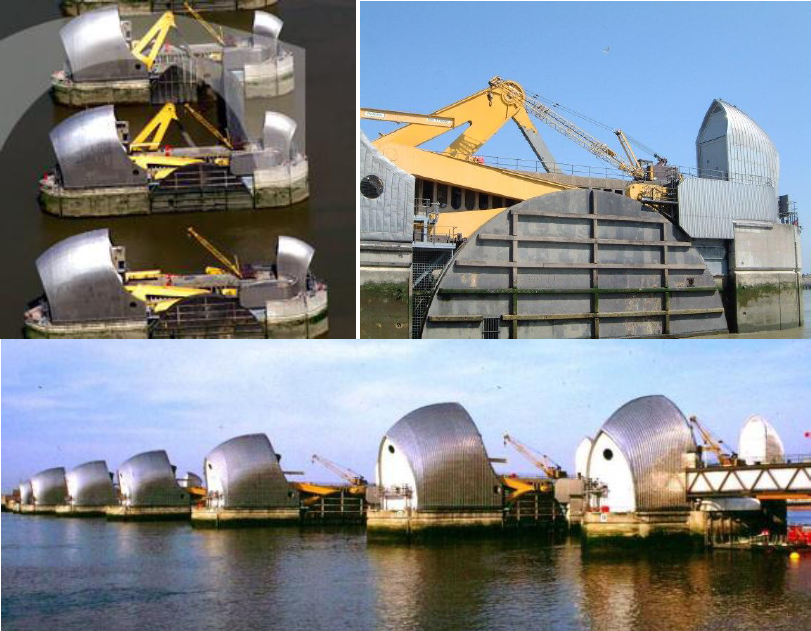
\includegraphics[width=.8\textwidth]{png/img1}
\end{center}

La barrière, mise en place sur la tamise depuis 1982, est longue de 520m et est constituée de
6 portes pivotantes actionnées par des vérins hydrauliques. Au repos, les portes 1 (voir schéma ci-après)
de forme circulaire reposent au fond de la tamise. Les plus grandes portes font 61 m de long
et 20 m de haut pour une masse de 3700 tonnes. Elles sont capables de supporter des charges de
plus de 9000 tonnes.

L'objectif est de calculer la vitesse de rotation des portes connaissant la vitesse de translation des
vérins dans la configuration dessinée. Les vérins sont alimentés sous une pression hydraulique de
valeur $P_{alim}$.
Données :
\begin{itemize}
\item La vitesse de translation de la tige du vérin 5 par rapport à 0 : $||\vect{V(D\in5/0)}||=5\cdot10^{-3} m/s$;
\item $CD=10,25m$;
\item toutes les liaisons sont supposées parfaites.
\end{itemize}
}

\subparagraph{}
\textit{En tenant compte de l'alimentation en énergie des vérins, tracer la vitesse de $\vectv{M}{4}{0}$.}

\subparagraph{}
\textit{Déterminer la vitesse de $\vectv{I}{3}{0}$.}
\ifthenelse{\boolean{prof}}{
\begin{corrige}
D'une part, $\vectv{I}{3}{0}=\vectv{I}{3}{4}+\vectv{I}{4}{0} = \vectv{I}{4}{0}$. 3 étant en liaison pivot de centre H par rapport 0, $\vectv{I}{3}{0}$ est perpendiculaire à $(HI)$. 

D'autre part, d'après la relation d'équiprojectivité, $\vectv{M}{4}{0}\cdot\vect{MI} = \vectv{I}{4}{0}\cdot\vect{MI}$. 

\end{corrige}
}{}

\subparagraph{}
\textit{Déterminer la vitesse de $\vectv{E}{2}{0}$.}
\ifthenelse{\boolean{prof}}{
\begin{corrige}
$\vectv{E}{3}{0} = \vectv{E}{2}{0}$ est perpendiculaire à $(EH)$. On détermine le vecteur en traçant le champ du vecteur vitesse. 

\end{corrige}
}{}


\subparagraph{}
\textit{Déterminer la vitesse de $\vectv{D}{1}{0}$.}
\ifthenelse{\boolean{prof}}{
\begin{corrige}
Tracé du vecteur vitesse par équiprojectivité. 

On a alors $||\vectv{D}{1}{0}||=34\cdot 10^{-3} \; m/s$.
\end{corrige}
}{}

\subparagraph{}
\textit{En déduire la valeur de la vitesse instantanée de rotation $\omega(1/0)$.}
\ifthenelse{\boolean{prof}}{
\begin{corrige}
$\omega(1/0) = \dfrac{||\vectv{D}{1}{0}||}{CD}=\dfrac{34\cdot 10^{-3}}{10,25}=3,33 \; rad/s$.
\end{corrige}
}{}

\subparagraph{}
\textit{Déterminer le centre instantané de rotation de 2 par rapport à 0.}
\ifthenelse{\boolean{prof}}{
\begin{corrige}
Le CIR de 2 par rapport à 0 est à l'instersection de :
\begin{itemize}
\item la perpendiculaire à $\vectv{D}{2}{0}$;
\item la perpendiculaire à $\vectv{E}{2}{0}$.
\end{itemize}

On peut aussi le théorème des 3 CIR alignés : 
\begin{itemize}
\item $I(2/0)$, $I(2/1)=D$ et $I(1/0)=C$ sont alignés;
\item $I(2/0)$, $I(2/3)=E$ et $I(3/0)=H$ sont alignés.
\end{itemize}

\end{corrige}
}{}

\ifthenelse{\boolean{prof}}{
\begin{center}
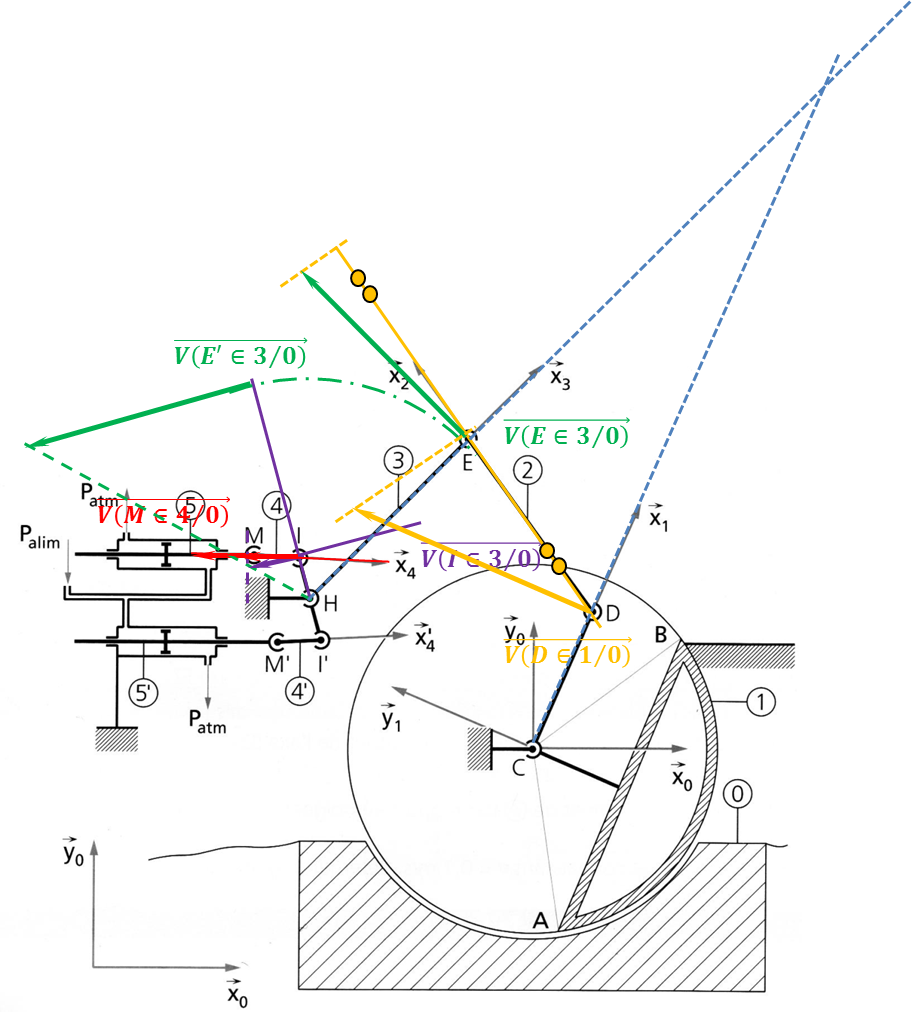
\includegraphics[width=.95\textwidth]{png/corrige_tamise1}

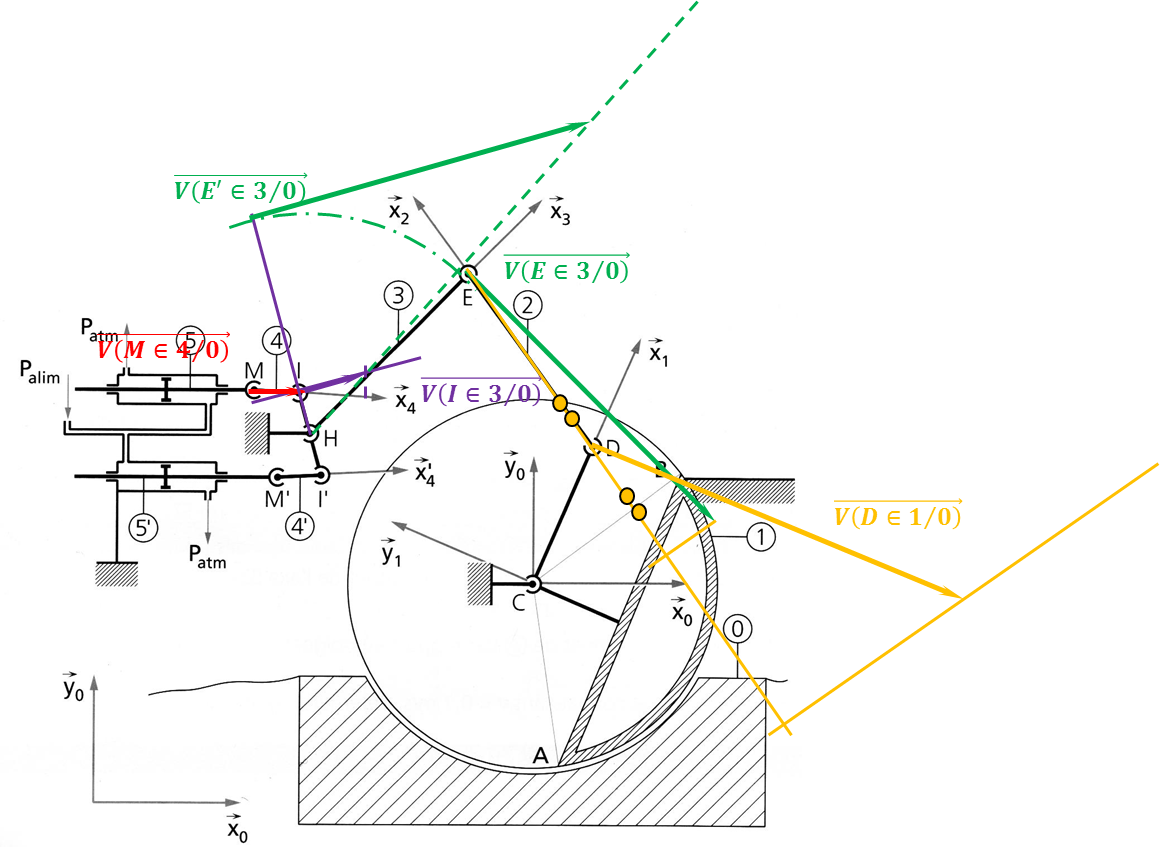
\includegraphics[width=.95\textwidth]{png/corrige_tamise}
\end{center}
}{}

\section*{Exercice 2}
\setcounter{subparagraph}{0}
Pour cet exercice, se référer au schéma du document réponse. 

L'objectif de ce mécanisme est de brider la pièce 1 en vu de son usinage. Le serrage est réalisé par le vérin (5 et 6). On donne $||\vectv{D}{5}{6}||=4\;cm/s$.

L'échelle sera de 1 cm pour 1 $cm/s$.

\subparagraph{}
\textit{Déterminer $\vectv{D}{5}{0}$.}
\ifthenelse{\boolean{prof}}{
\begin{corrige}
On a $\vectv{D}{5}{0}=\vectv{D}{5}{6}+\vectv{D}{6}{0} \Longleftrightarrow 
\vectv{D}{5}{6} = \vectv{D}{5}{0}-\vectv{D}{6}{0} $ :
\begin{itemize}
\item $\vectv{D}{5}{0}$ a une direction verticale;
\item $\vectv{D}{5}{6}$ est connu;
\item $\vectv{D}{6}{0}$ est perpendiculaire à la droite $(DE)$.
\end{itemize}

\end{corrige}
}{}


\subparagraph{}
\textit{Déterminer $||\vectv{A}{2}{0}||$.}
\ifthenelse{\boolean{prof}}{
\begin{corrige}
On a $\vectv{D}{5}{0}=\vectv{D}{5}{2}+\vectv{D}{2}{0}=\vectv{D}{2}{0}$.

Le CIR de $(2/0)$ est aligné avec le le CIR de $(3/2)=B$ et le CIR de $(2/0)=C$. Il appartient aussi à la droite perpendiculaire à $\vectv{D}{2}{0}$.

On peut alors utiliser le champ du vecteur vitesse. 

\end{corrige}
}{}

\ifthenelse{\boolean{prof}}{
\begin{center}
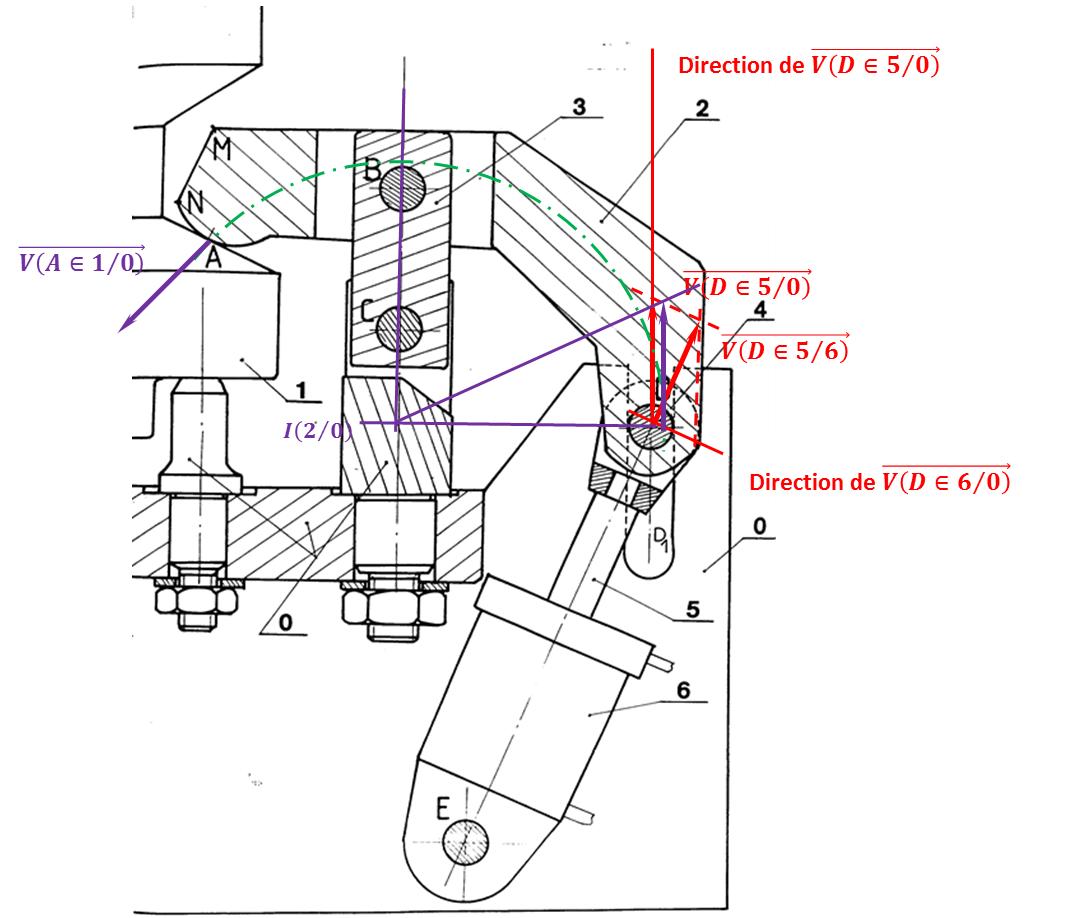
\includegraphics[width=.95\textwidth]{png/corrige_bride}
\end{center}
}{}





\section*{Exercice 3 : Etude du système de positionnement d'un appareil d'imagegerie médicale}
\setcounter{subparagraph}{0}

\ifthenelse{\boolean{prof}}{}{
\noindent\begin{minipage}[c]{.7\linewidth}

\indent L'étude porte sur un système permettant de réaliser des imageries médicales de vaisseaux sanguins sur un patient. Ce système conçu par General Electric Medical System, envoie des rayons X dans le corps du patient et mesure leur rayonnement. En fonction des informations reçues, une image de synthèse en 3 dimensions est réalisé en permettant de voir les éventuels problèmes médicaux à venir.
\end{minipage}\hfill
\begin{minipage}[c]{.2\linewidth}
\begin{center}
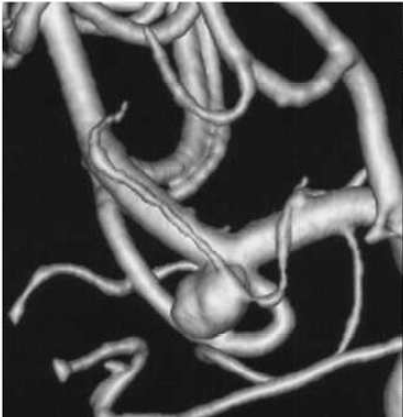
\includegraphics[width=.95\textwidth]{png/exo3_1}
\end{center}
\end{minipage}

\vspace{.25cm}

\begin{minipage}[c]{.4\linewidth}
\begin{center}
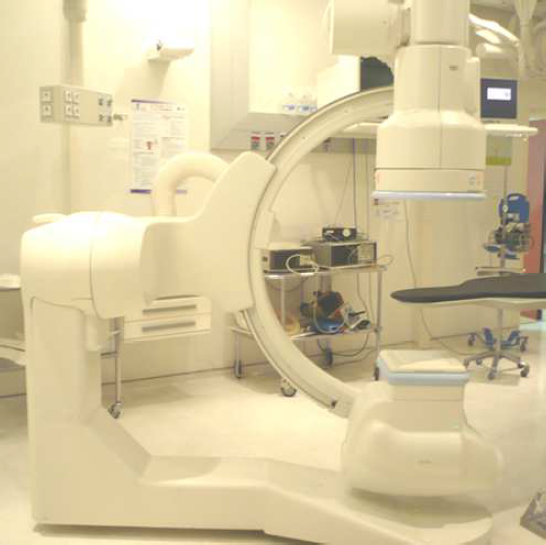
\includegraphics[height=5cm]{png/exo3_2}
\end{center}
\end{minipage}\hfill
\begin{minipage}[c]{.55\linewidth}
\begin{center}
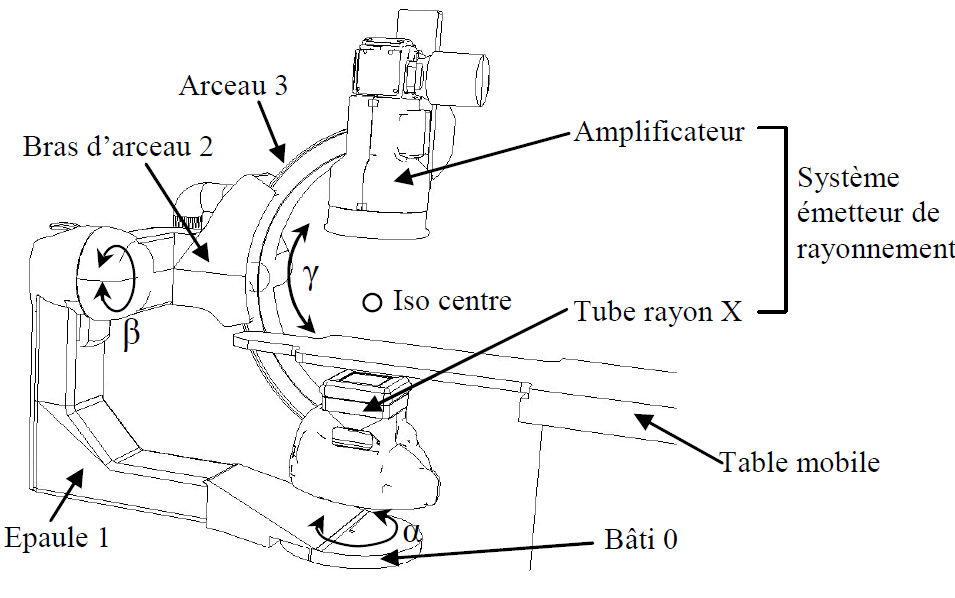
\includegraphics[height=6cm]{png/exo3_3}
\end{center}
\end{minipage}

\vspace{.25cm}

Ce système est constitué des éléments suivants : le bâti 0, une épaule 1 qui peut être mise en mouvement par rapport au bâti 0, un bras arceau 2 qui peut s'orienter par rapport à l'épaule 1 et un arceau 3 qui se déplace par rapport à bras d'arceau 2. Le patient est situé sur une table mobile. Le réglage en hauteur du patient sur la table mobile est possible pour son confor mais n'est pas utilisé au cours d'une analyse. Seuls les degrés de liberté $\alpha$, $\beta$ et $\gamma$ sont utilisés pendant l'analyse. L'émetteur de rayons, situé sur l'arceau, focalise la vision interne du patient en un point appelé iso centre.

\begin{center}
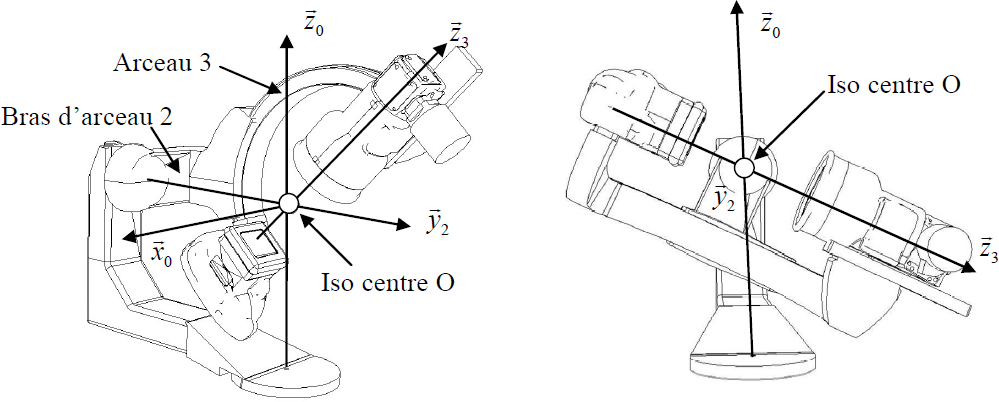
\includegraphics[height=6cm]{png/exo3_4}
\end{center}

Sur l'image de gauche, l'arceau 3 s'oriente par rapport au bras d'arceau 2 et sur l'image de droite le bras d'arceau 2 se déplace par rapport à l'épaule 1.
\vspace{.25cm}

%On donne ci-dessous un extrait de cahier des charges fonctionnel du système de positionnement dans la phase de vie correspondante à une mesure d'imagerie. 

%\subparagraph{}
%\textit{Déterminer le rapport de mouvements élémentaires utilisés (translation ou rotation) pour orienter le faisceau de rayon.}
\begin{minipage}[c]{.47\linewidth}
Conformément au cahier des charges, chaque axe élémentaire, piloté séparément, doit avoir une vitesse angulaire de $10\textdegree/s.$ en phase de mesure. Technologiquement, la chaîne d'action de chaque axe élémentaire est constituée d'un réducteur entre le moteur et l'effecteur. Ce réducteur diminue la vitesse angulaire d'un facteur 558. 
\end{minipage}\hfill
\begin{minipage}[c]{.47\linewidth}
\begin{center}
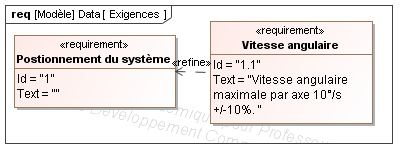
\includegraphics[width=.95\textwidth]{png/SysML/Exigences}
\end{center}
\end{minipage}
}

\subparagraph{}
\textit{Déterminer la vitesse angulaire de chaque moteur (en $tr/min$) qui permet de satisfaire le critère de vitesse angulaire du cahier des charges.}
\ifthenelse{\boolean{prof}}{
\begin{corrige}
$10\textdegree /s.\; \leftrightarrow \; 600\textdegree /min \; \leftrightarrow \; \dfrac{5}{3}\; tr/min.$ En prenant en compte le rapport de réduction, le moteur doit tourner à 930 tr/min.
\end{corrige}
}{}


\ifthenelse{\boolean{prof}}{}{
On s'intéresse à l'axe permettant de déplacer le bras d'arceau 2 par rapport à l'épaule 1. La structure de la chaîne fonctionnelle asservie de cet axe est la suivante :

\begin{center}
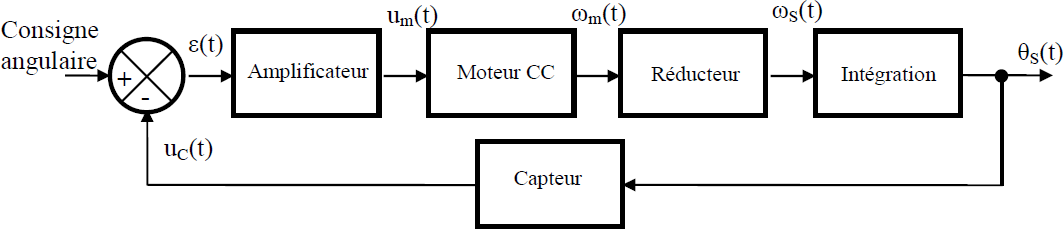
\includegraphics[width=.9\textwidth]{png/exo3_5}
\end{center}

Les différents éléments de cette chaîne fonctionnelle sont les suivants : 
\begin{itemize}
\item l'amplificateur est un gain pur $K_a$;
\item le réducteur est un gain pur $K_r$ (sans dimension);
\item le capteur est un gain pur $K_c$;
\item le moteur est un système d'ordre 1, de constante de temps $T_m$ et de gain $K_m$. On note la fonction de transfert du moteur $H_m(p)$.
\end{itemize}
}
\subparagraph{}
\textit{Déterminer la valeur numérique du bloc du réducteur $K_r$.}
\ifthenelse{\boolean{prof}}{
\begin{corrige}
$K_r=1/558$.
\end{corrige}
}{}


\subparagraph{}
\textit{Déterminer la fonction de transfert de la chaîne directe $FTCD(p)$, la fonction de transfert en boucle ouverte $FTBO(p)$ et la fonction de transfert en boucle fermée $FTBF(p)$ de cet asservissement. Exprimer les résultats en fonction de $K_a$, $K_m$, $K_r$, $K_c$ et $T_m$.}
\ifthenelse{\boolean{prof}}{
\begin{corrige}
On a :
$$
FTCD(p) = \dfrac{\Theta_S(p)}{\varepsilon(p)}= K_a \cdot \dfrac{K_m}{1+T_m p} \cdot K_r \cdot \dfrac{1}{p} 
= \dfrac{K_mK_a K_r}{p\left( 1+T_m p \right)}
$$

$$
FTBO(p) = \dfrac{U_c(p)}{\varepsilon(p)}= \dfrac{K_mK_a K_rK_c}{p\left( 1+T_m p \right)}
$$

$$
FTBF(p) = \dfrac{\Theta_S(p)}{\Theta_C(p)}=  \dfrac{\dfrac{K_mK_a K_r}{p\left( 1+T_m p \right)}}{1+\dfrac{K_mK_a K_rK_c}{p\left( 1+T_m p \right)}}
=\dfrac{K_mK_a K_r}{p\left( 1+T_m p \right)+K_mK_a K_rK_c}
$$
\end{corrige}
}{}


\subparagraph{}
\textit{Montrer que la fonction de transfert en boucle fermée de ce système peut s'écrire sous la forme d'un deuxième ordre $\dfrac{K}{1+2\dfrac{z}{\omega_0}p+\dfrac{1}{\omega_0}p^2}$. Donner l'expression littérale de $K$, $z$, $\omega_0$ en fonction de $K_a$, $K_m$, $K_r$, $K_c$ et $T_m$.}
\ifthenelse{\boolean{prof}}{
\begin{corrige}
Directement :
$$
FTBF(p) = \dfrac{\Theta_S(p)}{\Theta_C(p)}
=  \dfrac{\dfrac{1}{K_c}}{1+\dfrac{p\left( 1+T_m p \right)}{K_mK_a K_rK_c}}
=  \dfrac{\dfrac{1}{K_c}}{1+\dfrac{p}{K_mK_a K_rK_c}+\dfrac{T_m}{K_mK_a K_rK_c}p^2}
$$
On a alors :
$$
\left\{
\begin{array}{l}
K=\dfrac{1}{K_c} \\
\dfrac{2z}{\omega_0} = \dfrac{1}{K_mK_a K_rK_c} \\
\omega_0 = \sqrt{\dfrac{K_mK_a K_rK_c}{T_m}}
\end{array}
\right.
\Rightarrow 
\left\{
\begin{array}{l}
K=\dfrac{1}{K_c} \\
z =  \dfrac{\omega_0}{2}  \dfrac{1}{K_mK_a K_rK_c}  = \sqrt{\dfrac{K_mK_a K_rK_c}{T_m}} \dfrac{1}{2K_mK_a K_rK_c} 
=\dfrac{1}{2\sqrt{T_mK_mK_a K_rK_c}}\\
\omega_0 = \sqrt{\dfrac{K_mK_a K_rK_c}{T_m}}
\end{array}
\right.
$$


\end{corrige}
}{}


\subparagraph{}
\textit{Déterminer la réponse du moteur $\omega_m(t)$ à une entrée en échelon de tension $u_m(t)$ de la forme $u_m(t)=U_0 u(t)$ ($U_0$ valant 10 V.). Exprimer le résultat en fonction de $U_0$, $K_m$ et $T_m$.}
\ifthenelse{\boolean{prof}}{
\begin{corrige}
On a directement :  $\omega_m(t)=U_0K_m\left( 1-e^{-\dfrac{t}{T_m}}\right)\cdot u(t)$ .
\end{corrige}
}{}


\subparagraph{}
\textit{La réponse du système à cette entrée en échelon de tension $u_m(t)=10\cdot u(t)$ a été mesurée en sortie du réducteur. On donne la courbe obtenue. Déterminer les valeurs numériques expérimentales de $K_m$ et $T_m$.} %Réaliser les tracés utiles sur le document réponse.}
\ifthenelse{\boolean{prof}}{
\begin{corrige}
On a $K_m=2$. En utilisant la méthode des 62\% de la valeur finale, $T_m \simeq 0,03 s$.
\end{corrige}
}{}

\ifthenelse{\boolean{prof}}{}{
\begin{center}
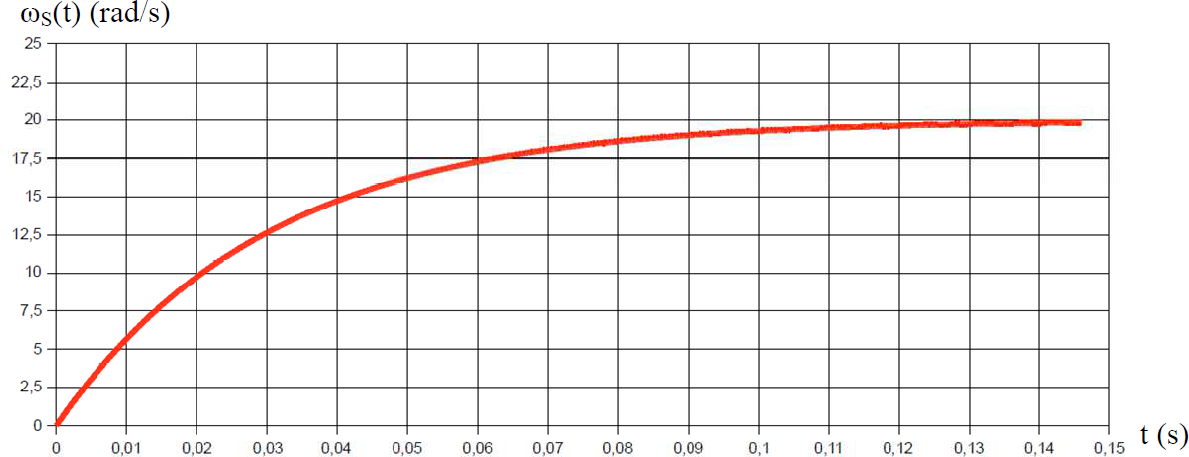
\includegraphics[width=.9\textwidth]{png/exo3_dr1}
\end{center}


Avec les valeurs numériques des coefficients des différents gains, on peut déterminer la valeur numérique de la fonction de transfert en boucle ouverte : $FTBO(p)=\dfrac{10}{p\left(1+\dfrac{1}{30}p \right)}$.
}

\subparagraph{}
\textit{Tracer les diagrammes de Bode asymptotiques de la fonction de transfert en boucle ouverte sur le document réponse 2. }
\ifthenelse{\boolean{prof}}{
\begin{corrige}
\begin{center}
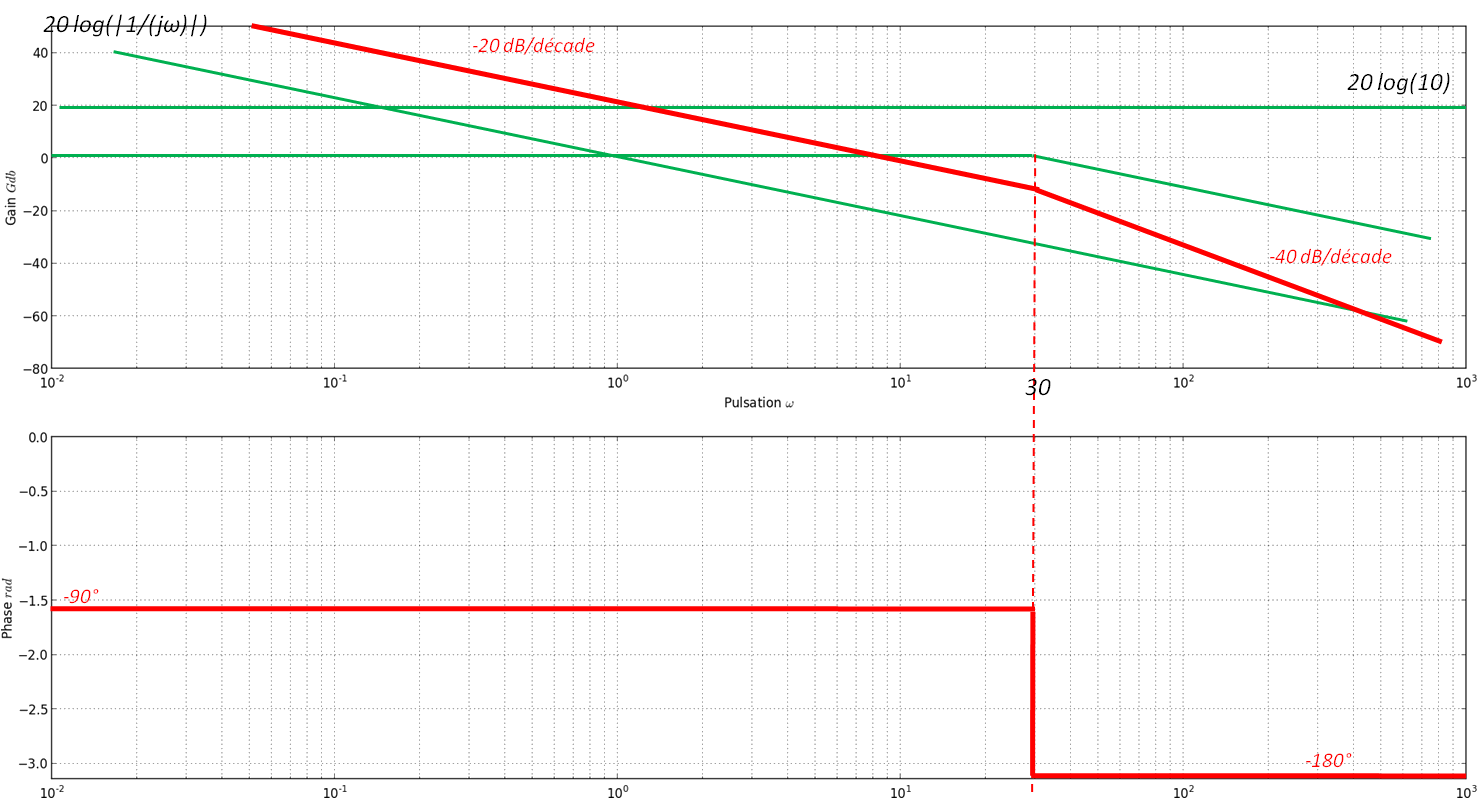
\includegraphics[width=.9\textwidth]{png/corrige_bode}
\end{center}
\end{corrige}
}{}


\subparagraph{}
\textit{Calculer le gain et la phase exacts pour $\omega=30\; rad/s$.}
\ifthenelse{\boolean{prof}}{
\begin{corrige}
On a 
$$AdB (\omega)= 20 \log_{10} (10) - 20 \log_{10}\sqrt{\omega^2}-20\log_{10}\sqrt{1^2 + \dfrac{\omega^2}{30^2}}
$$
Par ailleurs 
$$
\varphi(\omega)
 = \text{Arg} (10) -  \text{Arg} j\omega - \text{Arg}\left(1+\dfrac{1}{30} j\omega \right)
 = 0 - \dfrac{\pi}{2} - \arctan{\dfrac{\omega}{30}}
$$
On a donc $AdB (30) = -12,5 dB$ et $\varphi(30)=-2,356\; rad = -135 \textdegree$.

\end{corrige}
}{}

\ifthenelse{\boolean{prof}}{}{
%\subparagraph{}
%\textit{}
\newpage

\section*{Document réponse -- NOM :}
\subsection*{Exercice 1}
Représentation graphique des vitesses : $1 \; cm$ pour $2,5\cdot10^{-3} \; m/s$

\vfill

\begin{center}
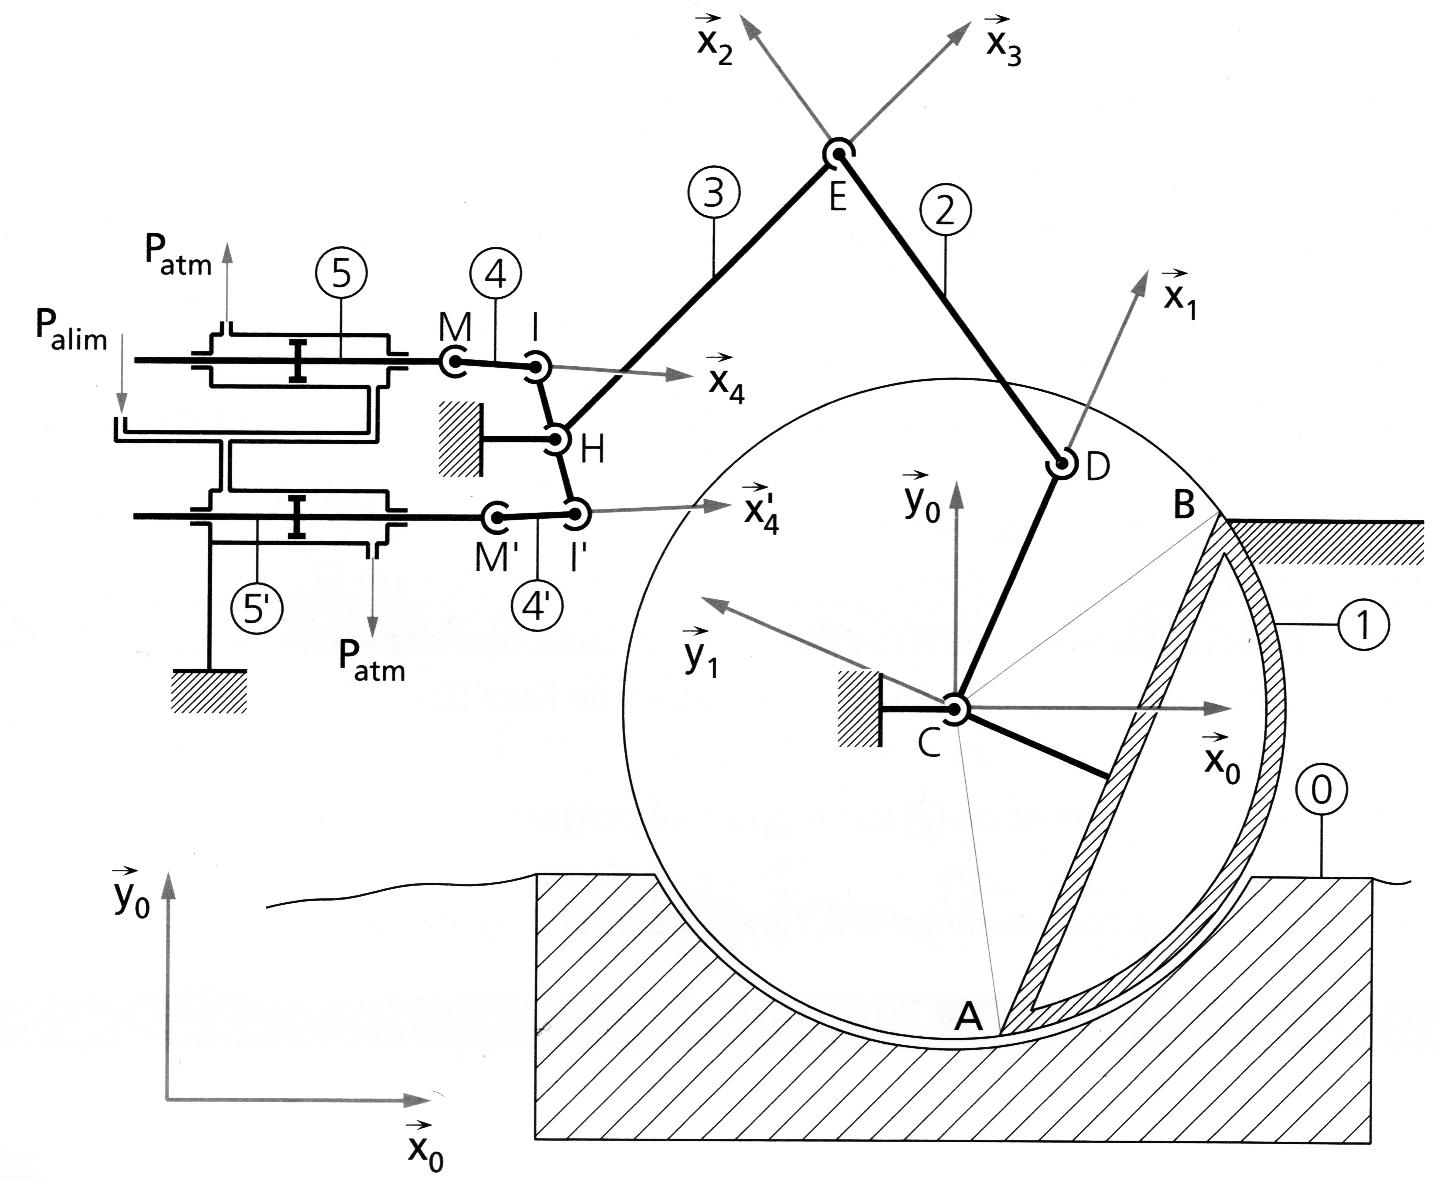
\includegraphics[width=.9\textwidth]{png/img2}
\end{center}

\newpage

\subsection*{Exercice 2}
\vfill
\begin{center}
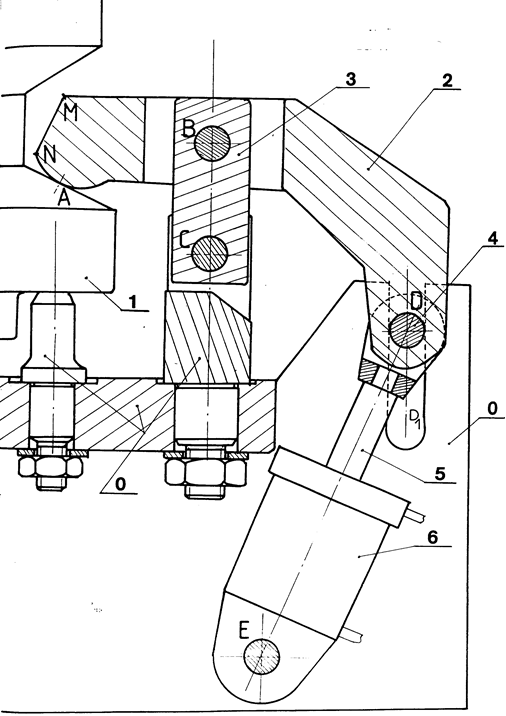
\includegraphics[width=.6\textwidth]{png/bride}
\end{center}

\newpage

\subsection*{Exercice 3}
\begin{center}
\rotatebox{90}{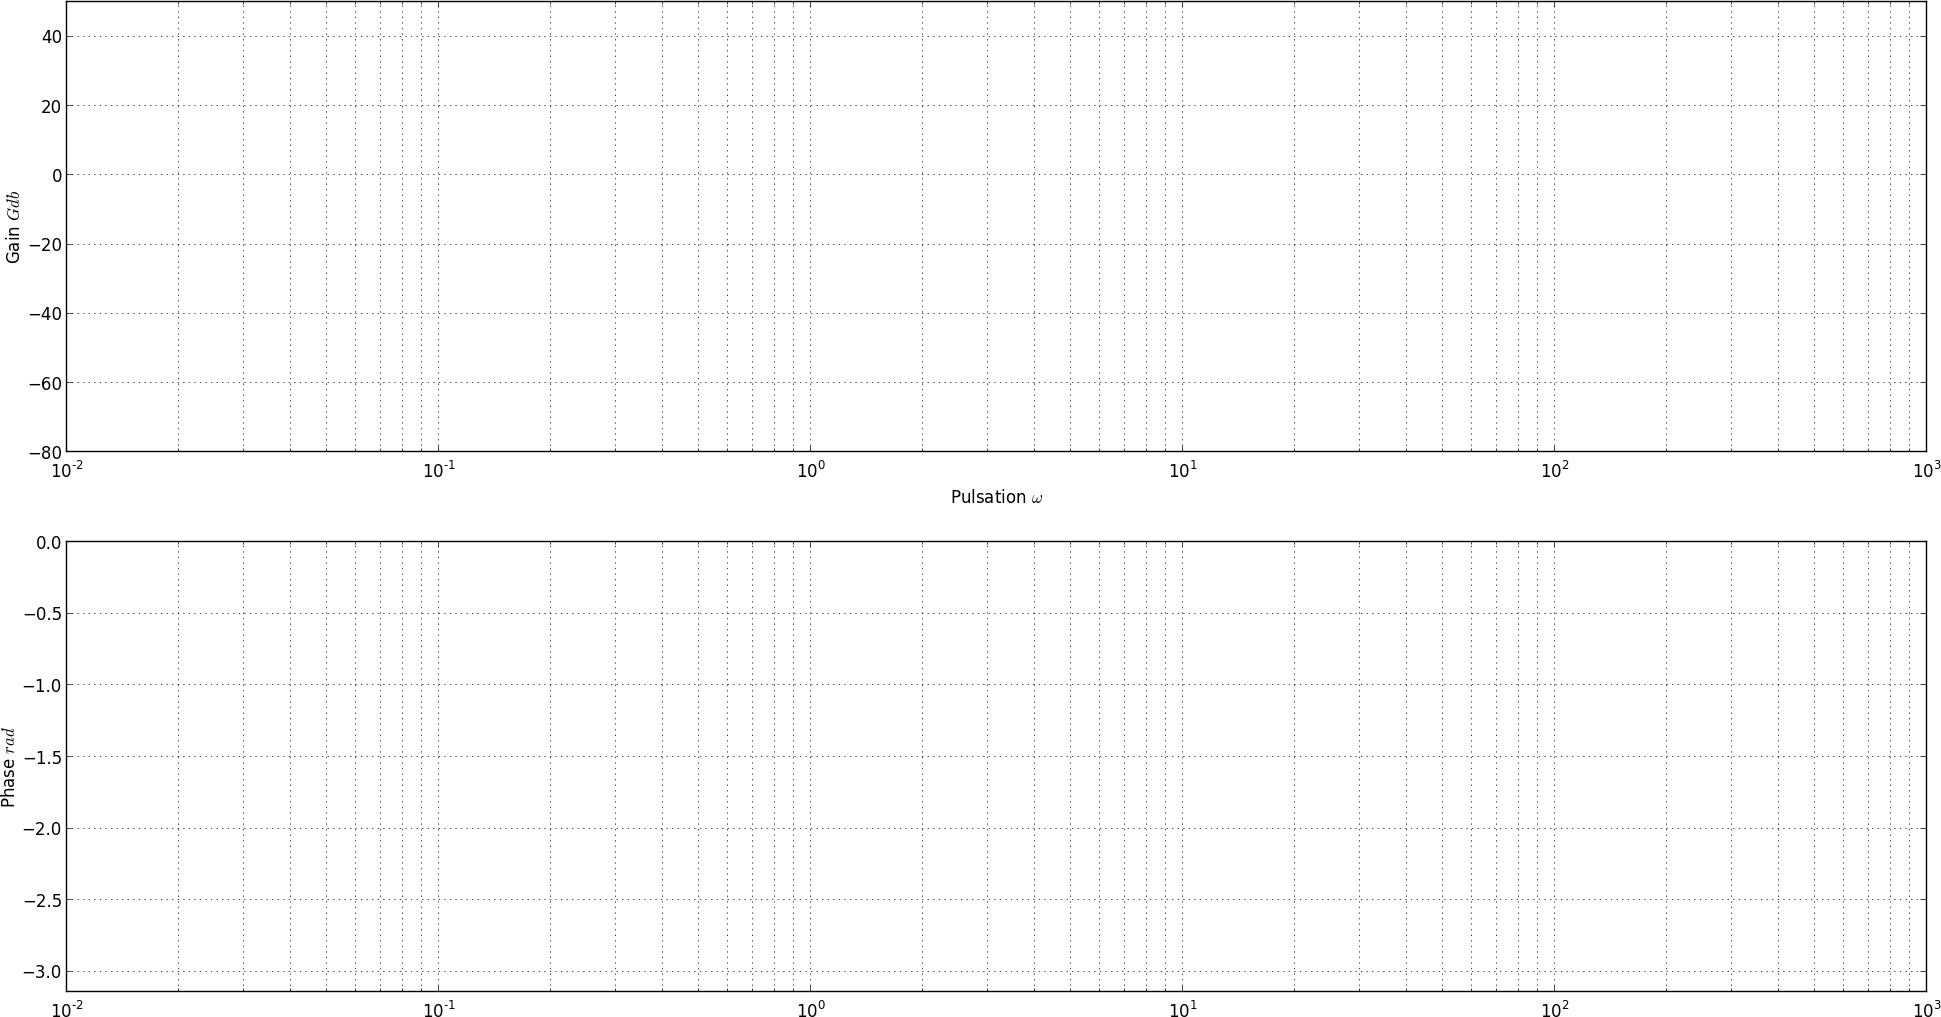
\includegraphics[width=.95\textheight]{png/figure_1}}
\end{center}
}%fin booleen prof
\end{document}
